% (C) Marc Lijour, 2016-2017
% Licensed under a Creative Commons License BY-SA
% https://creativecommons.org/licenses/by-sa/2.5/ca/
% Presentation for the Small Business Digitization Initiative (SBDI) training program
% see http://www.ictc-ctic.ca/small-business-digitization-initiative/ 
% authored by Marc Lijour, December 2016
% for the session running from January 2017 to September 2017
% 
% Variables
% TODO set the variables
% ---------------------- USER-DEFINED --------------------------------
\newcommand{\SFLtitle}{Digitization~Theory~Bonus}
\newcommand{\SFLlongtitle}{Other topics of interest}
\newcommand{\SFLsubtitle}{Small Business Digitization Initiative (SBDI) - Bonus}
\newcommand{\SFLauthor}{Marc~Lijour}
\newcommand{\SFLdate}{January 26, 2017}
\newcommand{\SFLsubject}{Digitization Theory}
% --------------------------------------------------------------------
% Template
% (C) Savoir-faire Linux, 2016 (this document and associated logos and art)
% This document is licensed under a Creative Commons License BY-SA (feel free to use the code, but all rights are reserved for logos and art)
% https://creativecommons.org/licenses/by-sa/2.5/ca/
% Savoir-faire Linux presentation template for LaTeX
% authored by Marc Lijour, December 2016
% This template comes with a first page on a blue background
% Possible improvement in future iterations
% - Test and fix as needed to work on xetex (to use Ubuntu fonts)
% === USAGE===
% Create a file for your LaTeX content (slides, etc), in which you must do the following:
% TODO 1 - set variables defined below
% TODO 2 - include this code by calling: % (C) Savoir-faire Linux, 2016 (this document and associated logos and art)
% This document is licensed under a Creative Commons License BY-SA (feel free to use the code, but all rights are reserved for logos and art)
% https://creativecommons.org/licenses/by-sa/2.5/ca/
% Savoir-faire Linux presentation template for LaTeX
% authored by Marc Lijour, December 2016
% This template comes with a first page on a blue background
% Possible improvement in future iterations
% - Test and fix as needed to work on xetex (to use Ubuntu fonts)
% === USAGE===
% Create a file for your LaTeX content (slides, etc), in which you must do the following:
% TODO 1 - set variables defined below
% TODO 2 - include this code by calling: % (C) Savoir-faire Linux, 2016 (this document and associated logos and art)
% This document is licensed under a Creative Commons License BY-SA (feel free to use the code, but all rights are reserved for logos and art)
% https://creativecommons.org/licenses/by-sa/2.5/ca/
% Savoir-faire Linux presentation template for LaTeX
% authored by Marc Lijour, December 2016
% This template comes with a first page on a blue background
% Possible improvement in future iterations
% - Test and fix as needed to work on xetex (to use Ubuntu fonts)
% === USAGE===
% Create a file for your LaTeX content (slides, etc), in which you must do the following:
% TODO 1 - set variables defined below
% TODO 2 - include this code by calling: \input{sfl-presentation-template-blue-EN}
% TODO 3 - Start the document as usual and you're in business; just use \begin{document} and don't forget to conclude with \end{document}
% TODO 4 - Use the custom method \SFLcoverpage instead of \titlepage to create your cover page
% Voilà!
%
\documentclass{beamer}
\usepackage{etoolbox}
% Variables
% ---------------------- USER-DEFINED --------------------------------
\ifdef{\SFLtitle}{}{\newcommand{\SFLtitle}{\color{red}Title TBD}}
\ifdef{\SFLlongtitle}{}{\newcommand{\SFLlongtitle}{\color{red}Long title TBD}}
\ifdef{\SFLsubtitle}{}{\newcommand{\SFLsubtitle}{\color{red}Subtitle TBD}}
\ifdef{\SFLauthor}{}{\newcommand{\SFLauthor}{\color{red}Author TBD}}
\ifdef{\SFLdate}{}{\newcommand{\SFLdate}{\color{red}Date TBD}}
\ifdef{\SFLsubject}{}{\newcommand{\SFLsubject}{\color{red}Subject TBD}}
% --------------------------------------------------------------------
\usetheme{Boadilla}
% Set color close to Savoir-faire Linux standard
\definecolor{beamer@blendedblue}{RGB}{86,176,201}
% Cover Page
\title[\SFLtitle] {\SFLlongtitle}
\subtitle{\SFLsubtitle}
\author{\SFLauthor}
\date{\SFLdate}
\subject{\SFLsubject}
\usepackage{tikz}
% -- possible approach through modif of the template (abandonned for now)
%\addtobeamertemplate{title page}{
%    \tikz[remember picture,overlay]
%        \node at ([xshift=0cm,yshift=0cm]current page.center) 
%		 {
\includegraphics[width=\paperwidth, height=\paperheight]{./images/sfl-background-blue}};
%}{}
%\setbeamercolor{title page}{fg=white}
%\setbeamercolor{titlelike}{fg=white}
%\setbeamertemplate{navigation symbols}{}
% Try Xetex to use system fonts (pdflatex makes it hard to import a font)
%\usepackage{fontspec}
%\setsansfont{Ubuntu}
%\setmonofont{Ubuntu Mono}
%
%\usepackage[absolute,overlay]{textpos}
%\setlength{\TPHorizModule}{\paperwidth}
%\setlength{\TPVertModule}{\paperheight}
% -- create a custom (command) title page -which has the benefit of not affecting the settings for the rest of the presentation
\newcommand{\SFLcoverpage}{\frame[plain]{
	\tikz[remember picture,overlay] {
        	\node(bkgd) at ([xshift=0cm,yshift=0cm]current page.center) 
			{
\includegraphics[width=\paperwidth, height=\paperheight]{../templates/images/sfl-background-blue}};
        	\node(logo) at ([xshift=0cm,yshift=2.5cm]current page.center) 
		 	{
\includegraphics[scale=.20]{../templates/images/logo-sfl-blanc-rgb-72dpi}};
	}
	\tikz[remember picture,overlay] {
        	\node(title) at ([xshift=0cm,yshift=1cm]current page.center) 
			{\Large\color{white}\textbf{{\SFLlongtitle}}};
        	\node(subtitle) at ([xshift=0cm,yshift=.2cm]current page.center) 
			{\small\color{white}\emph{\SFLsubtitle}};
        	\node(author) at ([xshift=0cm,yshift=-2cm]current page.center) 
			{\small\color{white}By~\SFLauthor};
        	\node(date) at ([xshift=0cm,yshift=-2.5cm]current page.center) 
			{\tiny\color{white}\SFLdate};
        	\node(footnote) at ([xshift=0cm,yshift=-4cm]current page.center) 
			{\TINY\color{white}\emph{The registered trademark Linux$^\circledR$ is used pursuant to a sublicense from LMI, the exclusive licensee of Linus Torvalds, owner of the mark on a world-wide basis.}};
    	}
}}
%
% This sets a Savoir-faire Linux logo at the bottom right corner of each page
\logo{
\includegraphics[scale=.1]{../templates/images/logo-sfl-250.png}}
\AtBeginSection[]
{
  \begin{frame}
    \frametitle{Table of Contents}
    \tableofcontents[currentsection]
  \end{frame}
}
%\usepackage[format=plain,justification=raggedright,singlelinecheck=false]{caption}
\usepackage[format=plain,justification=justified,singlelinecheck=false]{caption}
\usepackage[utf8]{inputenc}
\usepackage{dirtytalk}
\usepackage{wrapfig}
\usepackage{hyperref}
\usepackage{verbatim}
\usepackage{mathabx}
%\usepackage{MnSymbol}


% TODO 3 - Start the document as usual and you're in business; just use \begin{document} and don't forget to conclude with \end{document}
% TODO 4 - Use the custom method \SFLcoverpage instead of \titlepage to create your cover page
% Voilà!
%
\documentclass{beamer}
\usepackage{etoolbox}
% Variables
% ---------------------- USER-DEFINED --------------------------------
\ifdef{\SFLtitle}{}{\newcommand{\SFLtitle}{\color{red}Title TBD}}
\ifdef{\SFLlongtitle}{}{\newcommand{\SFLlongtitle}{\color{red}Long title TBD}}
\ifdef{\SFLsubtitle}{}{\newcommand{\SFLsubtitle}{\color{red}Subtitle TBD}}
\ifdef{\SFLauthor}{}{\newcommand{\SFLauthor}{\color{red}Author TBD}}
\ifdef{\SFLdate}{}{\newcommand{\SFLdate}{\color{red}Date TBD}}
\ifdef{\SFLsubject}{}{\newcommand{\SFLsubject}{\color{red}Subject TBD}}
% --------------------------------------------------------------------
\usetheme{Boadilla}
% Set color close to Savoir-faire Linux standard
\definecolor{beamer@blendedblue}{RGB}{86,176,201}
% Cover Page
\title[\SFLtitle] {\SFLlongtitle}
\subtitle{\SFLsubtitle}
\author{\SFLauthor}
\date{\SFLdate}
\subject{\SFLsubject}
\usepackage{tikz}
% -- possible approach through modif of the template (abandonned for now)
%\addtobeamertemplate{title page}{
%    \tikz[remember picture,overlay]
%        \node at ([xshift=0cm,yshift=0cm]current page.center) 
%		 {
\includegraphics[width=\paperwidth, height=\paperheight]{./images/sfl-background-blue}};
%}{}
%\setbeamercolor{title page}{fg=white}
%\setbeamercolor{titlelike}{fg=white}
%\setbeamertemplate{navigation symbols}{}
% Try Xetex to use system fonts (pdflatex makes it hard to import a font)
%\usepackage{fontspec}
%\setsansfont{Ubuntu}
%\setmonofont{Ubuntu Mono}
%
%\usepackage[absolute,overlay]{textpos}
%\setlength{\TPHorizModule}{\paperwidth}
%\setlength{\TPVertModule}{\paperheight}
% -- create a custom (command) title page -which has the benefit of not affecting the settings for the rest of the presentation
\newcommand{\SFLcoverpage}{\frame[plain]{
	\tikz[remember picture,overlay] {
        	\node(bkgd) at ([xshift=0cm,yshift=0cm]current page.center) 
			{
\includegraphics[width=\paperwidth, height=\paperheight]{../templates/images/sfl-background-blue}};
        	\node(logo) at ([xshift=0cm,yshift=2.5cm]current page.center) 
		 	{
\includegraphics[scale=.20]{../templates/images/logo-sfl-blanc-rgb-72dpi}};
	}
	\tikz[remember picture,overlay] {
        	\node(title) at ([xshift=0cm,yshift=1cm]current page.center) 
			{\Large\color{white}\textbf{{\SFLlongtitle}}};
        	\node(subtitle) at ([xshift=0cm,yshift=.2cm]current page.center) 
			{\small\color{white}\emph{\SFLsubtitle}};
        	\node(author) at ([xshift=0cm,yshift=-2cm]current page.center) 
			{\small\color{white}By~\SFLauthor};
        	\node(date) at ([xshift=0cm,yshift=-2.5cm]current page.center) 
			{\tiny\color{white}\SFLdate};
        	\node(footnote) at ([xshift=0cm,yshift=-4cm]current page.center) 
			{\TINY\color{white}\emph{The registered trademark Linux$^\circledR$ is used pursuant to a sublicense from LMI, the exclusive licensee of Linus Torvalds, owner of the mark on a world-wide basis.}};
    	}
}}
%
% This sets a Savoir-faire Linux logo at the bottom right corner of each page
\logo{
\includegraphics[scale=.1]{../templates/images/logo-sfl-250.png}}
\AtBeginSection[]
{
  \begin{frame}
    \frametitle{Table of Contents}
    \tableofcontents[currentsection]
  \end{frame}
}
%\usepackage[format=plain,justification=raggedright,singlelinecheck=false]{caption}
\usepackage[format=plain,justification=justified,singlelinecheck=false]{caption}
\usepackage[utf8]{inputenc}
\usepackage{dirtytalk}
\usepackage{wrapfig}
\usepackage{hyperref}
\usepackage{verbatim}
\usepackage{mathabx}
%\usepackage{MnSymbol}


% TODO 3 - Start the document as usual and you're in business; just use \begin{document} and don't forget to conclude with \end{document}
% TODO 4 - Use the custom method \SFLcoverpage instead of \titlepage to create your cover page
% Voilà!
%
\documentclass{beamer}
\usepackage{etoolbox}
% Variables
% ---------------------- USER-DEFINED --------------------------------
\ifdef{\SFLtitle}{}{\newcommand{\SFLtitle}{\color{red}Title TBD}}
\ifdef{\SFLlongtitle}{}{\newcommand{\SFLlongtitle}{\color{red}Long title TBD}}
\ifdef{\SFLsubtitle}{}{\newcommand{\SFLsubtitle}{\color{red}Subtitle TBD}}
\ifdef{\SFLauthor}{}{\newcommand{\SFLauthor}{\color{red}Author TBD}}
\ifdef{\SFLdate}{}{\newcommand{\SFLdate}{\color{red}Date TBD}}
\ifdef{\SFLsubject}{}{\newcommand{\SFLsubject}{\color{red}Subject TBD}}
% --------------------------------------------------------------------
\usetheme{Boadilla}
% Set color close to Savoir-faire Linux standard
\definecolor{beamer@blendedblue}{RGB}{86,176,201}
% Cover Page
\title[\SFLtitle] {\SFLlongtitle}
\subtitle{\SFLsubtitle}
\author{\SFLauthor}
\date{\SFLdate}
\subject{\SFLsubject}
\usepackage{tikz}
% -- possible approach through modif of the template (abandonned for now)
%\addtobeamertemplate{title page}{
%    \tikz[remember picture,overlay]
%        \node at ([xshift=0cm,yshift=0cm]current page.center) 
%		 {
\includegraphics[width=\paperwidth, height=\paperheight]{./images/sfl-background-blue}};
%}{}
%\setbeamercolor{title page}{fg=white}
%\setbeamercolor{titlelike}{fg=white}
%\setbeamertemplate{navigation symbols}{}
% Try Xetex to use system fonts (pdflatex makes it hard to import a font)
%\usepackage{fontspec}
%\setsansfont{Ubuntu}
%\setmonofont{Ubuntu Mono}
%
%\usepackage[absolute,overlay]{textpos}
%\setlength{\TPHorizModule}{\paperwidth}
%\setlength{\TPVertModule}{\paperheight}
% -- create a custom (command) title page -which has the benefit of not affecting the settings for the rest of the presentation
\newcommand{\SFLcoverpage}{\frame[plain]{
	\tikz[remember picture,overlay] {
        	\node(bkgd) at ([xshift=0cm,yshift=0cm]current page.center) 
			{
\includegraphics[width=\paperwidth, height=\paperheight]{../templates/images/sfl-background-blue}};
        	\node(logo) at ([xshift=0cm,yshift=2.5cm]current page.center) 
		 	{
\includegraphics[scale=.20]{../templates/images/logo-sfl-blanc-rgb-72dpi}};
        	\node(CC-BY-SA) at ([xshift=5cm,yshift=-3.5cm]current page.center) 
			{\href{https://creativecommons.org/licenses/by-sa/2.5/ca/}{
\includegraphics[scale=.4]{../templates/images/CC-BY-SA-403x141}}};
	}
	\tikz[remember picture,overlay] {
        	\node(title) at ([xshift=0cm,yshift=1cm]current page.center) 
			{\Large\color{white}\textbf{{\SFLlongtitle}}};
        	\node(subtitle) at ([xshift=0cm,yshift=.2cm]current page.center) 
			{\small\color{white}\emph{\SFLsubtitle}};
        	\node(author) at ([xshift=0cm,yshift=-2cm]current page.center) 
			{\small\color{white}By~\SFLauthor};
        	\node(date) at ([xshift=0cm,yshift=-2.5cm]current page.center) 
			{\tiny\color{white}\SFLdate};
        	\node(footnote) at ([xshift=0cm,yshift=-4cm]current page.center) 
			{\TINY\color{white}\emph{The registered trademark Linux$^\circledR$ is used pursuant to a sublicense from LMI, the exclusive licensee of Linus Torvalds, owner of the mark on a world-wide basis.}};
    	}
}}
%
% This sets a Savoir-faire Linux logo at the bottom right corner of each page
\logo{
	
\includegraphics[scale=.1]{../templates/images/logo-sfl-250.png}
}
\AtBeginSection[]
{
  \begin{frame}
    \frametitle{Table of Contents}
    \tableofcontents[currentsection]
  \end{frame}
}
%\usepackage[format=plain,justification=raggedright,singlelinecheck=false]{caption}
\usepackage[format=plain,justification=justified,singlelinecheck=false]{caption}
\usepackage[utf8]{inputenc}
\usepackage{dirtytalk}
\usepackage{wrapfig}
\usepackage{hyperref}
\usepackage{verbatim}
\usepackage{mathabx}
%\usepackage{MnSymbol}


% Extra packages
\usepackage{amssymb}
\usepackage{amsmath}
\usepackage[american]{babel}
\usepackage{csquotes}
\usepackage[backend=biber,style=apa]{biblatex}
\DeclareLanguageMapping{american}{american-apa}
% Use one bib file per section
\addbibresource{references-privacy.bib}
%\addbibresource{references-XYZ.bib}
\definecolor{links}{HTML}{2A1B81}
\hypersetup{colorlinks,linkcolor=,urlcolor=links}
% Start of the document
\begin{document}
% Cover page
% Do not use this: \frame{\titlepage}
% use this instead:
\SFLcoverpage

% (C) Marc Lijour, 2016-2017 
% Licensed under a Creative Commons License BY-SA
% https://creativecommons.org/licenses/by-sa/2.5/ca/
% Presentation for the Small Business Digitization Initiative (SBDI) training program
% see http://www.ictc-ctic.ca/small-business-digitization-initiative/ 
% authored by Marc Lijour, December 2016
% for the session running from January 2017 to September 2017
% 
% ======================================================================================================
%                                      PRIVACY
% ======================================================================================================
\section{Privacy Matters}
% --------------------- Definition --------------------------
\subsection{Why it matters}
	\begin{frame}
	\frametitle{Devices for Digital Consumption}
	\framesubtitle{}
	        \begin{figure}[h]
                \centering
                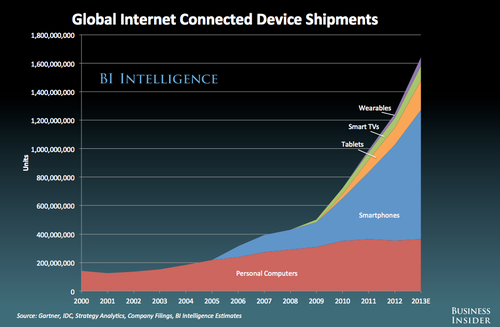
\includegraphics[width=.8\textwidth]{../pics/globalIOTDeviceShipments}
		\caption{Picture from \href{http://blog.kanyi.me/post/66994307568/contrarian-thinking-mobile-vs-pc-in-emerging}{\cite{kanyi}}}
        	\end{figure}
	\end{frame}

	\begin{frame}
	\frametitle{Microsoft's View on IoT by 2015}
	\framesubtitle{Devices sharing information about our lives}
	        \begin{figure}[h]
                \centering
                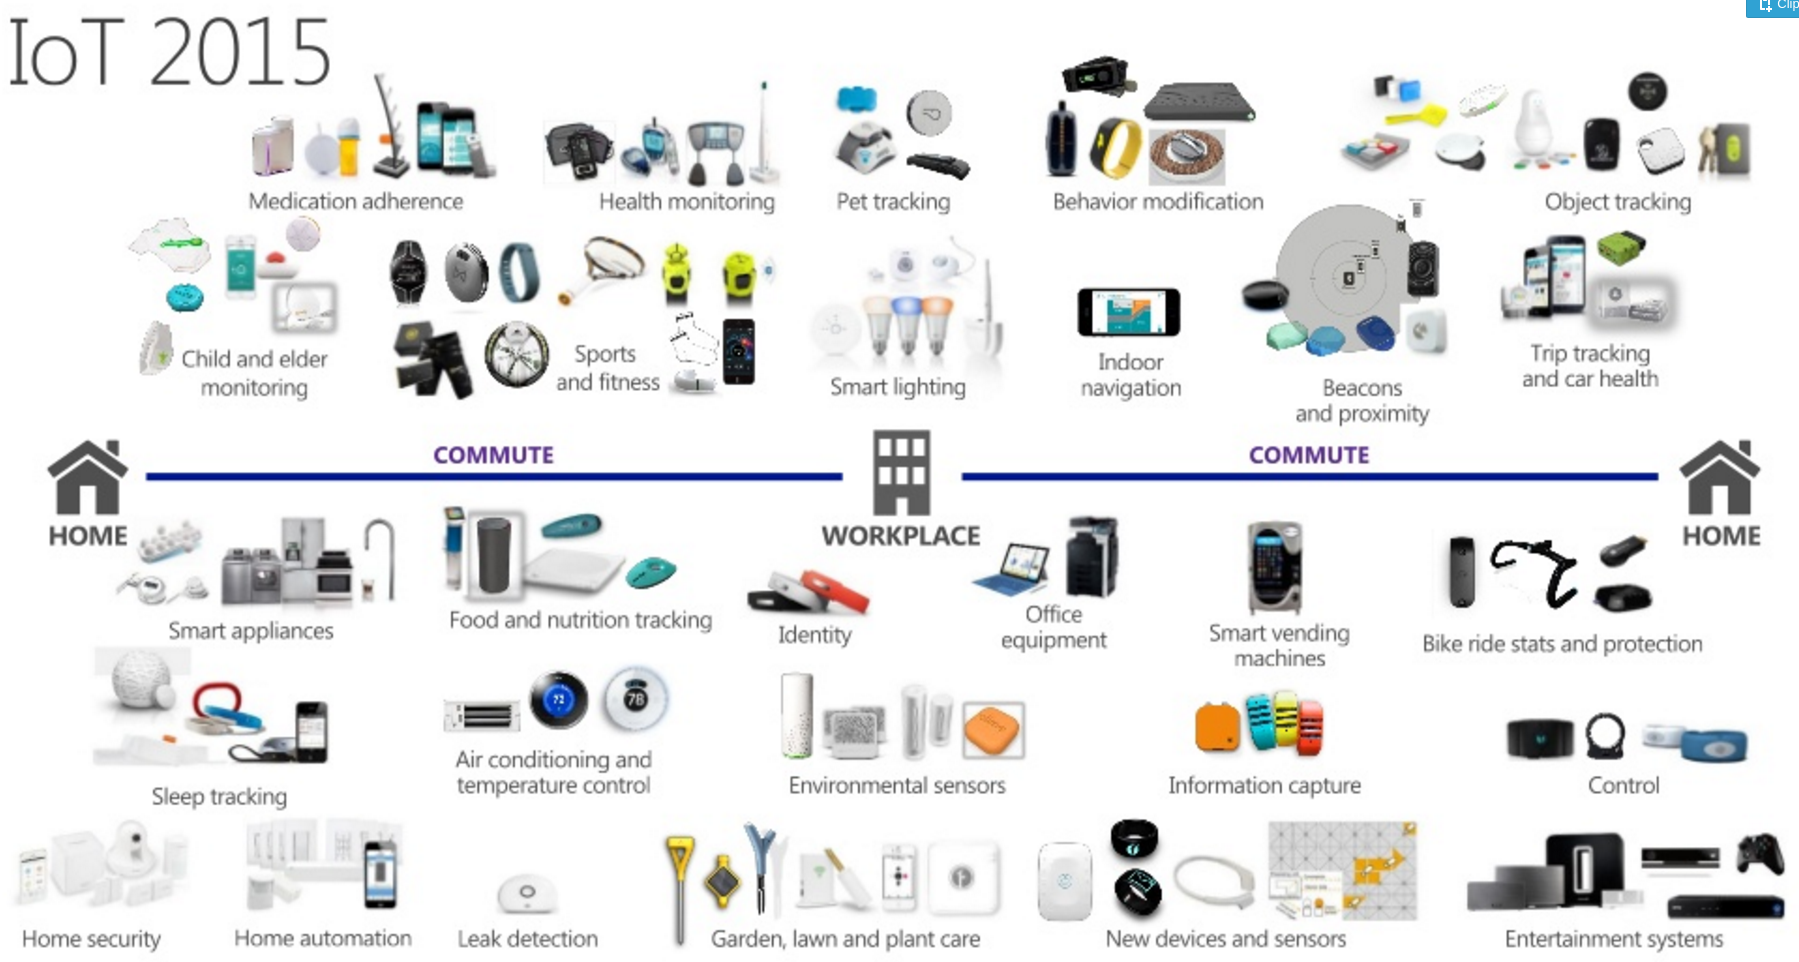
\includegraphics[width=.8\textwidth]{../pics/msft-IoT2015}
		\caption{IoT across devices with Windows 10 and Azure IoT Suite \href{http://www.slideshare.net/BosniaAgile/iot-across-devices-with-windows-10-and-azure-iot-suite-by-admir-tuzovi}{by \cite{admir}}}
        	\end{figure}
	\end{frame}

	\begin{frame}
	\frametitle{All our data is online}
	\framesubtitle{}
	        \begin{figure}[h]
                \centering
                
\includegraphics[width=.8\textwidth]{../pics/Cartoon_cloud.png}
        	\end{figure}
	\end{frame}

	\begin{frame}
	\frametitle{All our data is online}
	\framesubtitle{}
	        \begin{figure}[h]
                \centering
                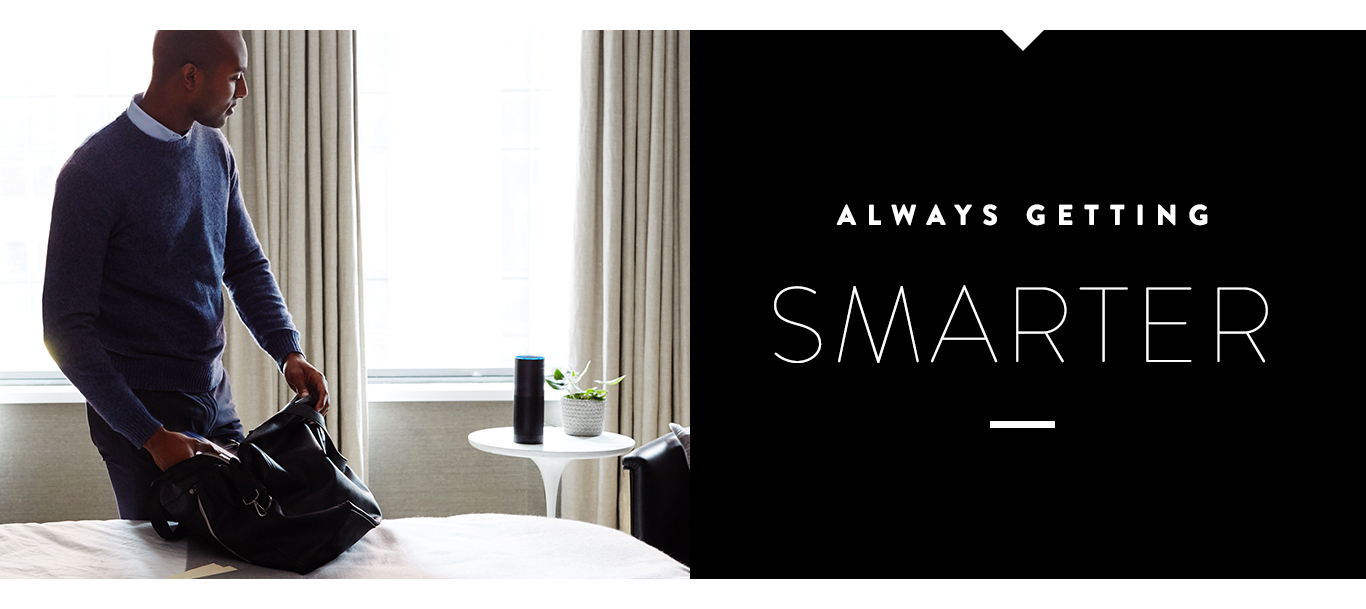
\includegraphics[width=.8\textwidth]{../pics/alexa-feature-smarter}
		\caption{\href{http://www.forbes.com/sites/tonybradley/2017/01/05/alexa-is-listening-but-amazon-values-privacy-and-gives-you-control/\#7c920725eed5}{The \textbf{AI} from Amazon is (almost) always listening, and the police is interested} (\cite{bradley2017})}
        	\end{figure}
	\end{frame}

	\begin{frame}
	\frametitle{What could go wrong?}
	\framesubtitle{(and should we trust government?)}
	        \begin{figure}[h]
                \centering
                
\includegraphics[width=.8\textwidth]{../pics/Trump_fingerup}
		\caption{\tiny\url{http://www.zerohedge.com/news/2016-08-08/trump-financial-plan}}
        	\end{figure}
	\end{frame}

	\frame{
	\frametitle{Canada has managed to stay on the safe side}
	\begin{figure}		
		\centering
		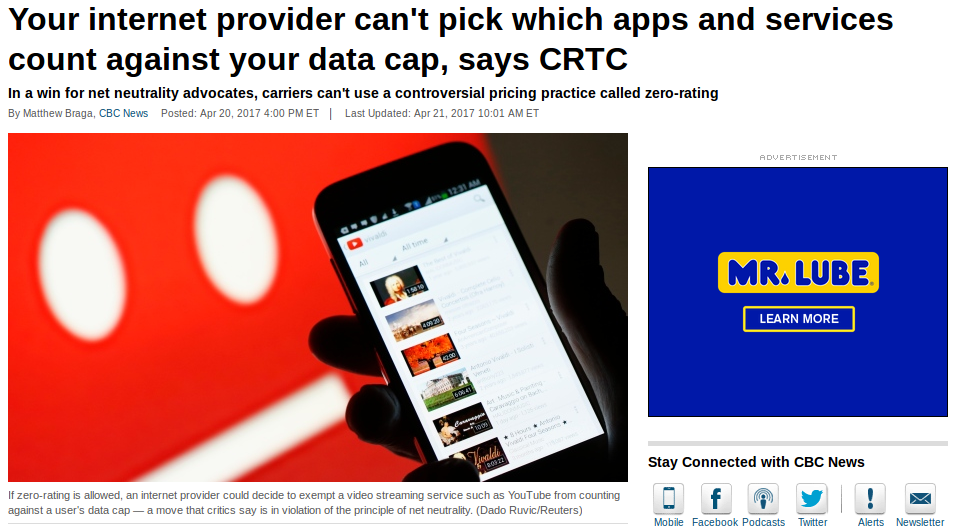
\includegraphics[width=.8\textwidth]{../pics/cbcnews20170420-netneutrality}
		\caption{\href{http://www.cbc.ca/news/technology/crtc-zero-rating-differential-pricing-decision-videtron-net-neutrality-2017-1.4077717}{see the recent article from CBC~News (\cite{cbcnews20170420})}\\and see \href{https://openmedia.org/en/openmedias-presentation-crtc-hearings-differential-pricing-aka-zero-rating}{\citeauthor{openmedia201704}'s presentation at the CRTC hearing (2016)}}
	\end{figure}
	}

%%%%%%%%%%%%%% 3rd SECTION: The Case for Freedom %%%%%%%%%%%%%%%%%
\section[Section]{Challenges to our Freedom}
	\begin{frame}
	\frametitle{The meaning of Freedom}
	\framesubtitle{}
		\begin{itemize}[<+->]
			\item Do what you like while respecting the next in kind's freedom
			\item Democracy
			\item Citizenship
			\item Human Rights
			\item Rule of Law (Justice, Equity)
			\item Liberté - Égalité - Fraternité
		\end{itemize}
	\end{frame}

	\begin{frame}
	\frametitle{What could go wrong?}
	\framesubtitle{Excessive (?) Government Surveillance \& Intervention}
		\begin{itemize}[<+->]
			\item Citizen Biometric Registry --a real perspective \href{http://www.pcworld.com/article/3139461/security/french-plan-for-biometric-database-of-60-million-people-sparks-outcry.html}{in France} (\cite{frbiometric})
			\item Patriot Act (\& others: French Govnt Act, 2015...)
			\item Chinese Firewall
			\item Government-led Cyberattacks
		\end{itemize}
	\end{frame}

	\begin{frame}
	\frametitle{The User is the Product}
	\framesubtitle{GAFAM \& Corporate Interests under scrutiny}
		\begin{outline}
%			\1 Google for example (see \href{http://www.forbes.com/sites/benkepes/2013/12/04/google-users-youre-the-product-not-the-customer/\#2871b0bc1624}{Forbes})
			\1 Users are the product (e.g. Google, according to \cite{forbes:google})
%			\1 Microsoft \href{http://www.businessinsider.com/microsoft-shuts-down-scroogled-website-2015-1}{'Scroogled' Campaign} in reaction
			\1 Microsoft launched a ``Scroogled'' campaign as a result (\cite{bi:microsoft}), but what about privacy issues in Windows~10 (\cite{zdnet:windows})?
			\1 In a case against Google, US Magistrate Judge Paul Grewal declared: "in this model, the users are the real product"
			\1 Follow the money:
				\2 US Internet Advertising Revenue in 2015: \$59.6 billion
				\2 Google: \$30 billion
				\2 Facebook: \$8 billion
			\1 Big Data \& Analytics is thriving with multiple data points (devices, apps, cameras...)
			\1 Organizations are vulnerable to security breaches
		\end{outline}
	\end{frame}


%%%%%%%%%%%%%% 4th SECTION: Solutions to saveguard Freedom %%%%%%%%%%%%%%%%%
\section[Section]{Working Efficiently AND (not OR) Protecting our Freedom}
	\begin{frame}
	\frametitle{Educate about Cybersecurity}
	\framesubtitle{Example: CyberTitan}
	\begin{columns}
		\column{0.5\textwidth}
			\begin{itemize}[<+->]
				\item ICTC program for high school students
				\item in partnership with the US Air Force Association’s CyberPatriot Program
				\item to develop in-demand skills needed to work in CyberSecurity, and other STEM areas
			\end{itemize}
		\column{0.5\textwidth}
	        	\begin{figure}[h]
                	\centering
                	
\includegraphics[width=.6\textwidth]{../pics/CP_Cybertitan1-150x150}
			\caption{\url{http://www.cybertitan.ca}}
        		\end{figure}
	\end{columns}
	\end{frame}

	\begin{frame}
	\frametitle{Support the OpenMedia's Net Neutrality Campaign}
	\framesubtitle{}
	        \begin{figure}[h]
                \centering
                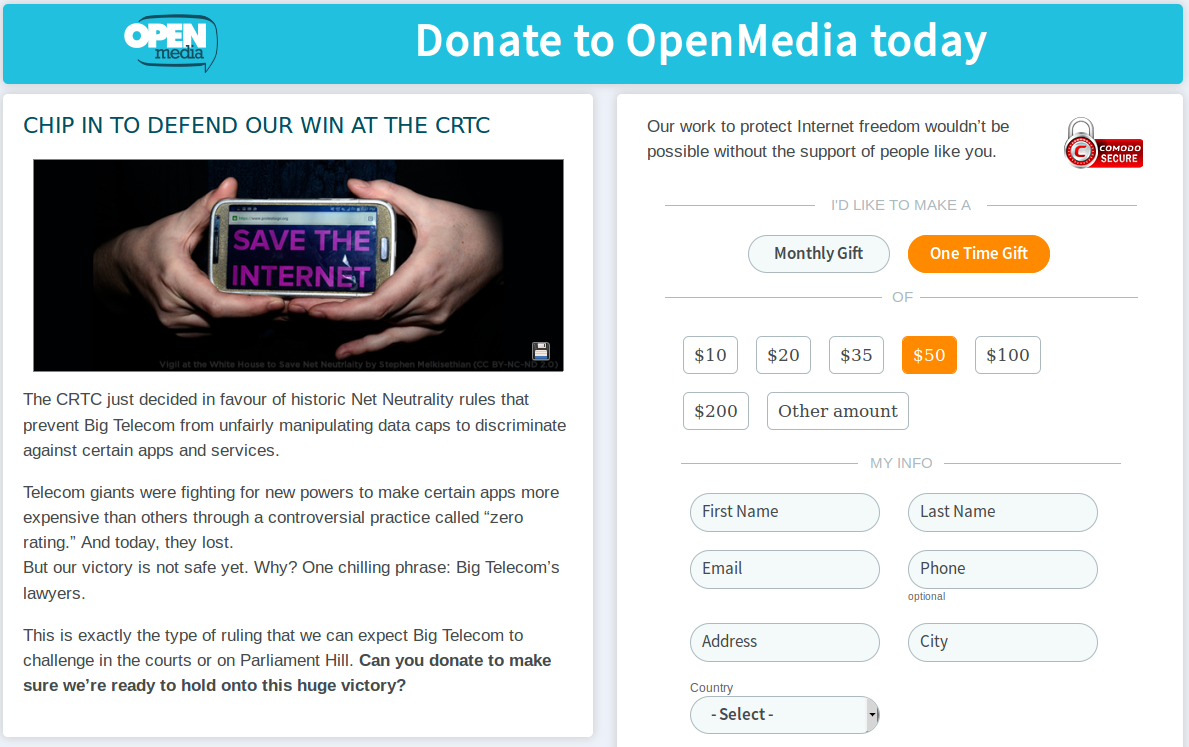
\includegraphics[width=.8\textwidth]{../pics/openmedia-donate-re-crtc}
		\caption{\url{https://act.openmedia.org/zerorating/donate/?src=161479}}
        	\end{figure}
	\end{frame}

	\begin{frame}
	\frametitle{Learn from Mozilla Internet Citizen}
	\framesubtitle{}
	        \begin{figure}[h]
                \centering
                
\includegraphics[width=.8\textwidth]{../pics/moz-Internet-citizen}
		\caption{\url{https://blog.mozilla.org/internetcitizen/}}
        	\end{figure}
	\end{frame}

	\begin{frame}
	\frametitle{Solve the toughest 21st Century Challenges with PIE\tiny\textsuperscript{\textregistered}}
	\framesubtitle{}
	        \begin{figure}[h]
                \centering
                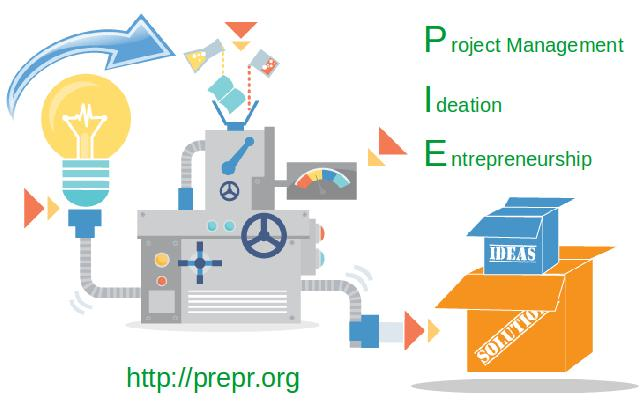
\includegraphics[width=.8\textwidth]{../pics/PIE_slide}
		\caption{\url{https://prepr.org}}
        	\end{figure}
	\end{frame}

	\begin{frame}
	\frametitle{Design your EdTech Environment with Privacy in Mind}
	\framesubtitle{}
	       	\begin{figure}[h]
               	\centering
               	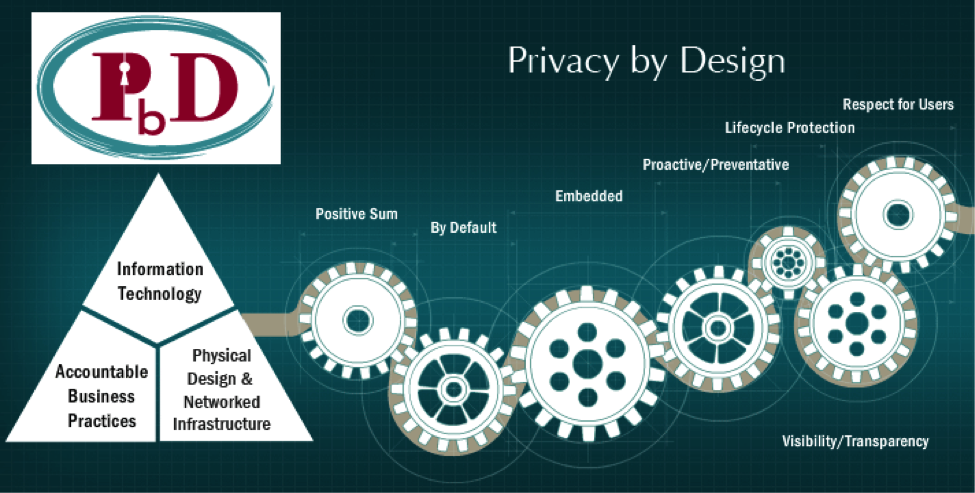
\includegraphics[width=.8\textwidth]{../pics/privacybydesign}
		\caption{Dr. Ann Cavoukian, Executive Director, \href{http://www.ryerson.ca/pbdi/privacy-by-design/certification/TheSevenFoundationalPrinciplesofPrivacybyDesign/}{Privacy and Big Data Institute (Dr.~\cite{cavoukian2011})}}
        	\end{figure}
	\end{frame}

	\begin{frame}
	\frametitle{Prefer Decentralized Systems that put you in control}
	\framesubtitle{Examples: Blockchain, and Ring for Secure Communications}
	        \begin{figure}[h]
                \centering
                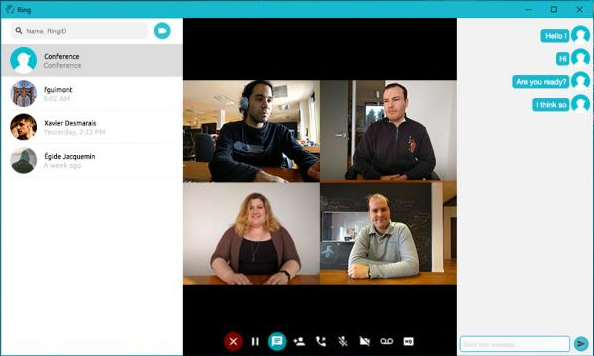
\includegraphics[width=.8\textwidth]{../pics/ring_interface_desktop}
		\caption{Data is shared as a need-to-know basis, see \url{http://ring.cx}}
        	\end{figure}
	\end{frame}

	\begin{frame}
	\frametitle{Build Community Clouds that you control}
	\framesubtitle{}
		\begin{itemize}[<+->]
			\item Hosted in Canada
			\item On your premises or at a secure location
			\item As a school board, or an association of privacy-conscious teachers
			\item As an individual (for example on OVH or Microsoft Azure)
			\item With the help of students 
		\end{itemize}
	\end{frame}

	\begin{frame}
	\frametitle{Secure Clouds for your Pocket Book}
	\framesubtitle{OVH is the Top 3 Cloud Company with a data centre in Canada}
	        \begin{figure}[h]
                \centering
                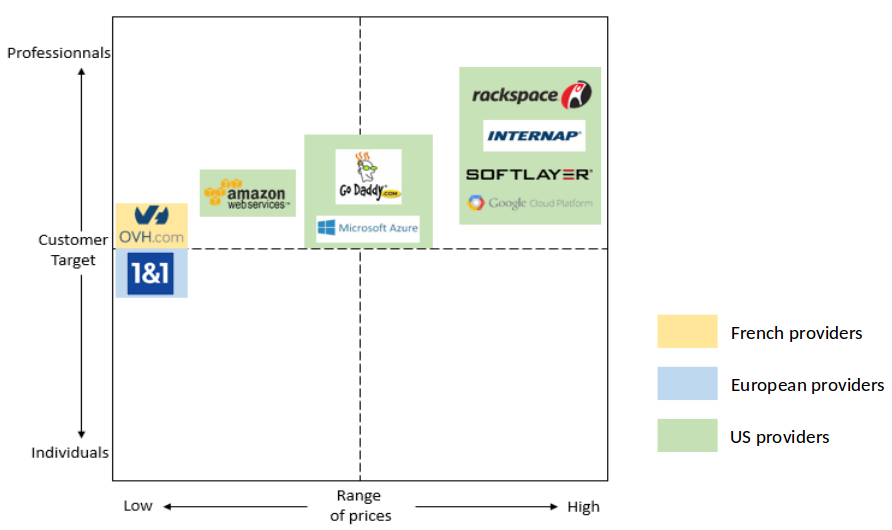
\includegraphics[width=.8\textwidth]{../pics/OVH-cloud-magic-quadrant}
        	\end{figure}
	\end{frame}

	\begin{frame}
	\frametitle{OVH in Canada}
	\framesubtitle{}
		\begin{outline}
			\1 +30M\$ invested in Canada since 2013 
			\1 +3,000 Customers in Canada
			\1 2 PoP in Canada (Montreal and Toronto) and 11 in the US
			\1 Strategic partnerships:
				\2 Rogers as a reseller of Public Cloud Enterprise solutions Canada-wide 
				\2 VMWare (Partner Innovation Award received in 2016)
				\2 OpenStack (one of the 3 major contributors WW)
			\1 Technological partners: \textbf{Savoir-faire-Linux}, LinkByNet...%, S3 Technologies, Globalia…
%			\1 Hundreds of customers served in 40 countries (Middle East, Asia, LATAM, USA\ldots)
		\end{outline}
	        \begin{figure}[h]
                \centering
                
\includegraphics[width=.8\textwidth]{../pics/OpenStack-Rogers-VMWare}
        	\end{figure}
	\end{frame}

	\begin{frame}
	\frametitle{OVH Global Footprint}
	\framesubtitle{\#1 in Europe, Top 3 Globally}
	        \begin{figure}[h]
                \centering
                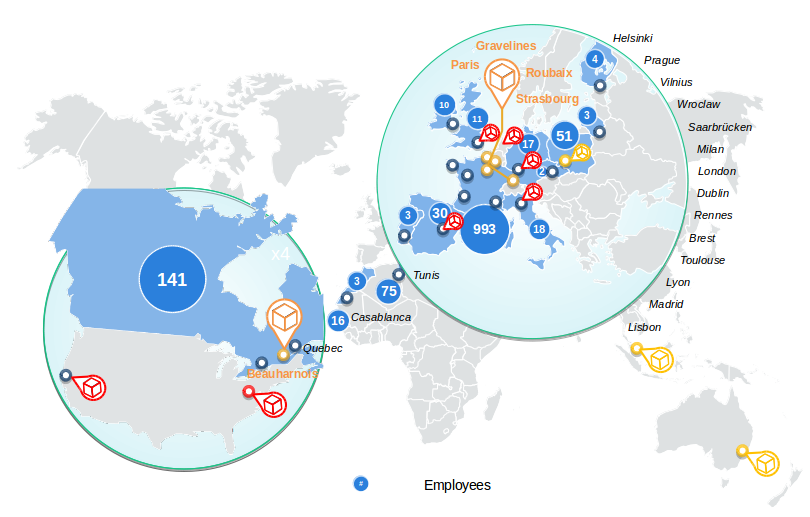
\includegraphics[width=.8\textwidth]{../pics/OVH-global_presence}
        	\end{figure}
	\end{frame}

	\begin{frame}
	\frametitle{Build your own server / IoT device}
	\framesubtitle{with lunch money}
	        \begin{figure}[h]
                \centering
                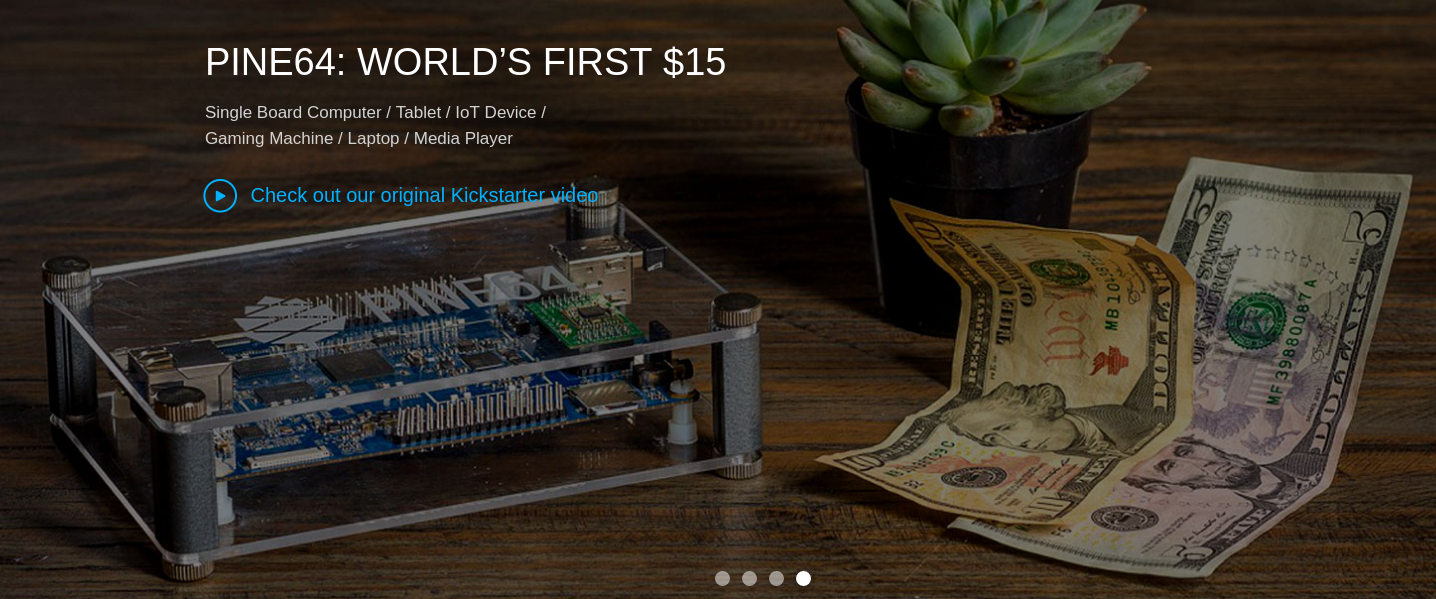
\includegraphics[width=.8\textwidth]{../pics/pine64}
		\caption{\url{https://www.pine64.org}}
        	\end{figure}
	\end{frame}

	\begin{frame}
	\frametitle{Build your own server / IoT device}
	\framesubtitle{on a coffee budget}
	        \begin{figure}[h]
                \centering
                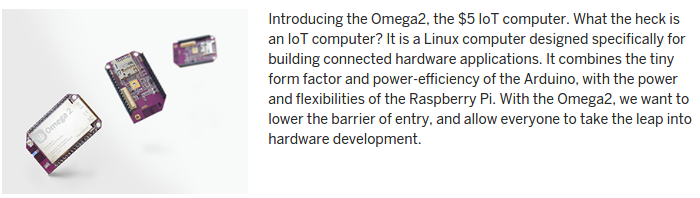
\includegraphics[width=.8\textwidth]{../pics/Omega2}
		\caption{\tiny{\url{https://www.indiegogo.com/projects/omega2-5-linux-computer-with-wi-fi-made-for-iot}}}
        	\end{figure}
%		\url{https://www.indiegogo.com/projects/omega2-5-linux-computer-with-wi-fi-made-for-iot}
	\end{frame}

	\begin{frame}
	\frametitle{Use Free Software Alternatives}
	\framesubtitle{Example: Framasoft alternative to \href{https://blog.google/topics/education/introducing-g-suite-education/}{G Suite for Education} \& other popular SaaS}
	\begin{columns}
		\column{0.5\textwidth}
	        	\begin{figure}[h]
               		\centering
                	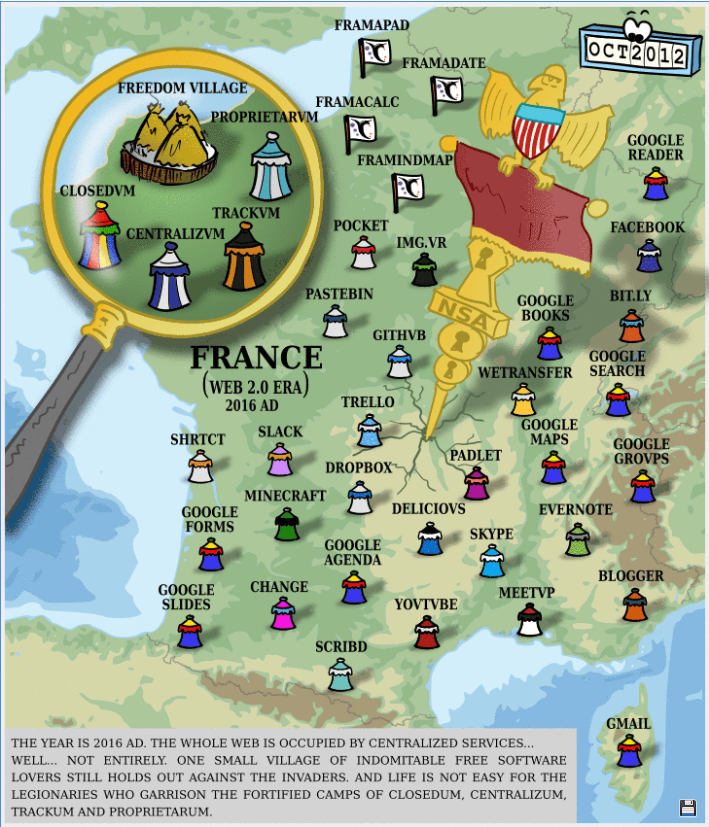
\includegraphics[width=.8\textwidth]{../pics/framasoft-gaulle}
        		\end{figure}
		\column{0.5\textwidth}
	        	\begin{figure}[h]
                	\centering
                	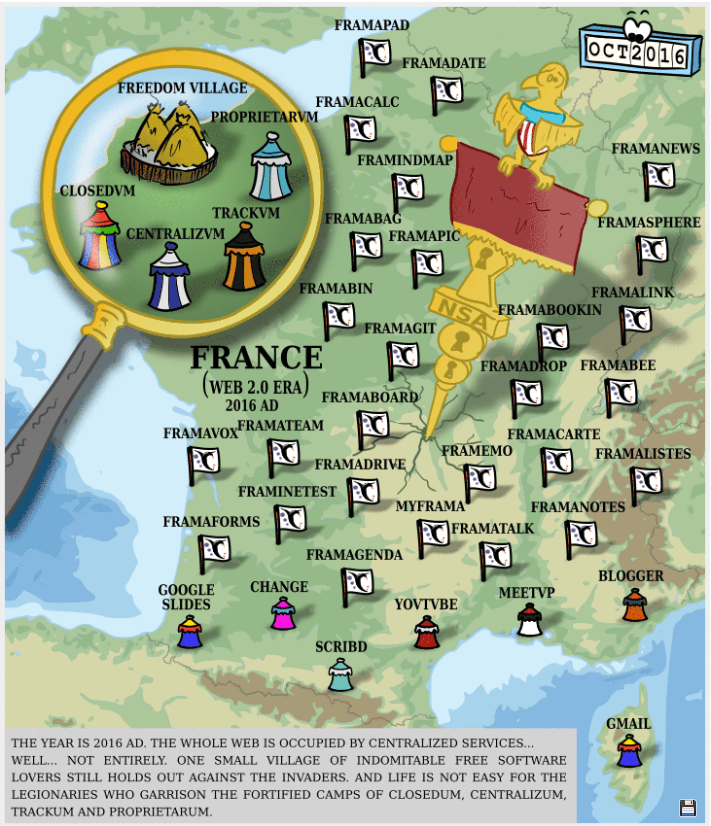
\includegraphics[width=.8\textwidth]{../pics/framasoft-gaulle-201610}
        		\end{figure}
	\end{columns}
	\end{frame}

	\begin{frame}
	\frametitle{Framasoft}
	\framesubtitle{\url{https://framasoft.org}}
		\begin{itemize}
			\item Founded in France (2004)
			\item Promotes and educates about Free Software, Free Culture, Free Services
			\item Flagship project to offer Free/Libre alternatives to dominant proprietary offers
			\item 3 FTEs, and a large community
			\item 30 solutions online (SaaS), or download and install on your own cloud/server
		\end{itemize}
	\end{frame}

	\begin{frame}
	\frametitle{30 Framasoft Services}
	\framesubtitle{}
	        \begin{figure}[h]
                \centering
                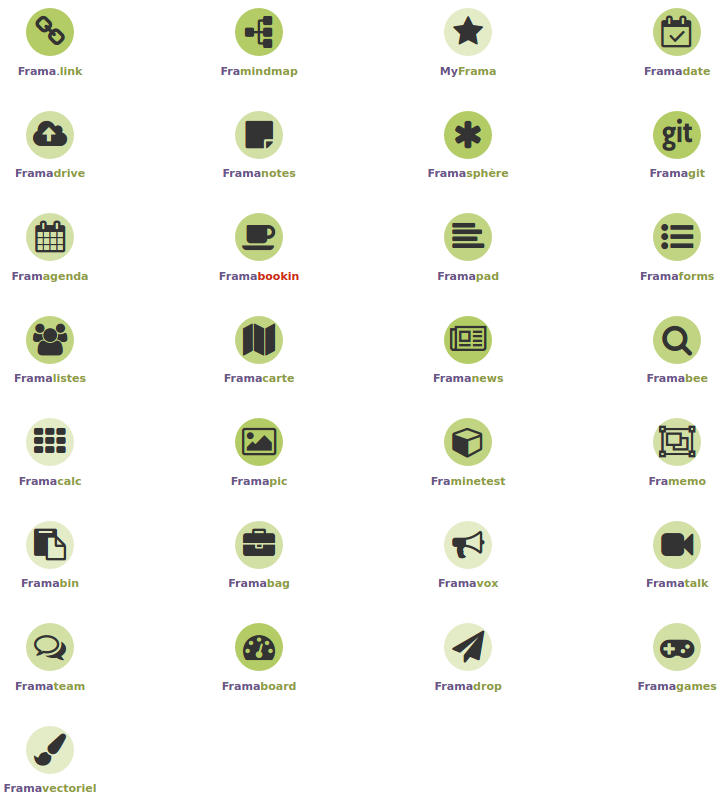
\includegraphics[width=.55\textwidth]{../pics/framasoft-solutions}
		\caption{\url{https://degooglisons-internet.org/liste?l=en}}
        	\end{figure}
	\end{frame}

	\begin{frame}
	\frametitle{Framadrive $\leftrightarrow$ Google Drive}
	\framesubtitle{}
	        \begin{figure}[h]
                \centering
                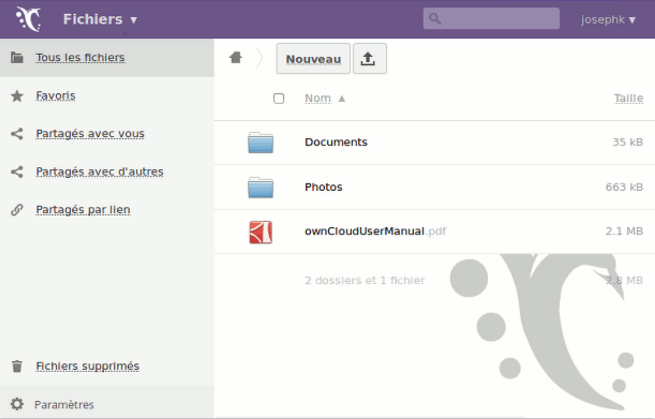
\includegraphics[width=.8\textwidth]{../pics/framadrive}
		\caption{Based on \href{https://owncloud.org/}{OwnCloud} -with calendars, contacts, mobile app...}
        	\end{figure}
	\end{frame}

	\begin{frame}
	\frametitle{Framacalc $\leftrightarrow$ Google Spreadsheet}
	\framesubtitle{}
	        \begin{figure}[h]
                \centering
                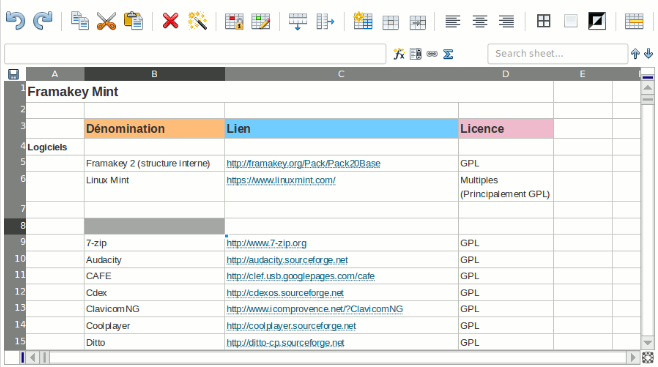
\includegraphics[width=.8\textwidth]{../pics/framacalc}
		\caption{Based on \href{https://ethercalc.net}{EtherCalc}}
        	\end{figure}
	\end{frame}

	\begin{frame}
	\frametitle{Framagenda $\leftrightarrow$ Google Calendar}
	\framesubtitle{}
	        \begin{figure}[h]
                \centering
                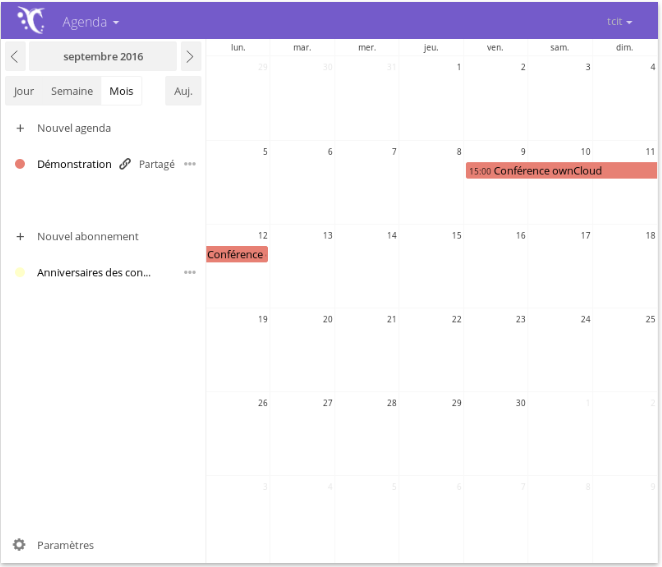
\includegraphics[width=.8\textwidth]{../pics/framagenda}
		\caption{Based on \href{https://nextcloud.com}{NextCloud}}
        	\end{figure}
	\end{frame}

	\begin{frame}
	\frametitle{Framadate $\leftrightarrow$ Doodle}
	\framesubtitle{}
	        \begin{figure}[h]
                \centering
                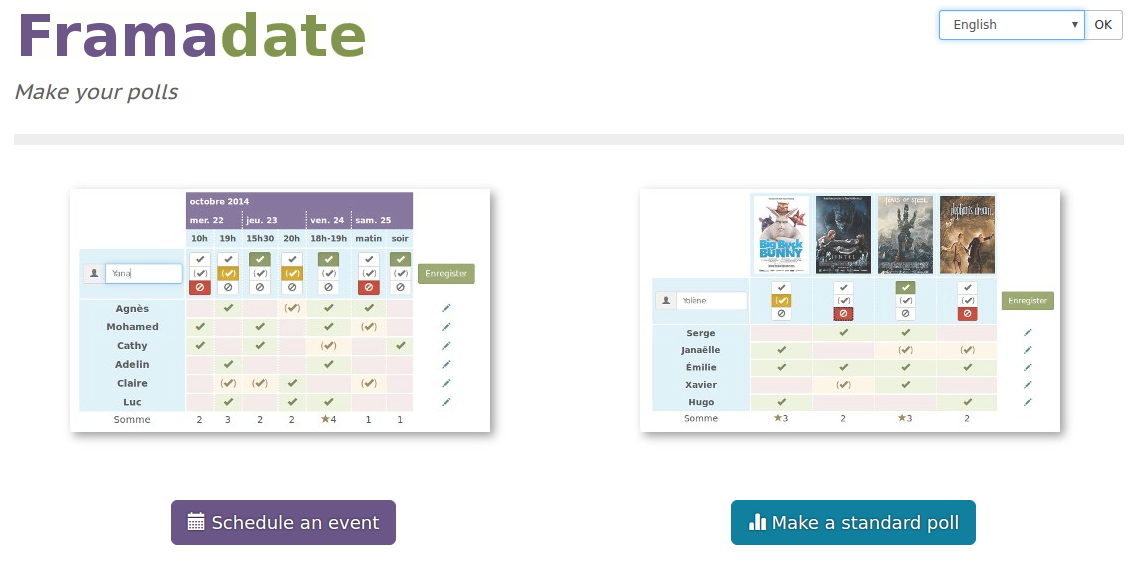
\includegraphics[width=.8\textwidth]{../pics/framadate}
        	\end{figure}
	\end{frame}

	\begin{frame}
	\frametitle{Framapad $\leftrightarrow$ Evernote}
	\framesubtitle{}
	        \begin{figure}[h]
                \centering
                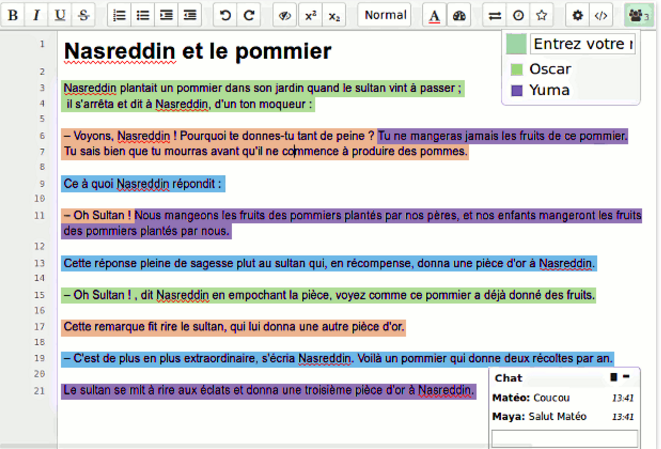
\includegraphics[width=.8\textwidth]{../pics/framapad}
        	\end{figure}
	\end{frame}

	\begin{frame}
	\frametitle{Framacarte: Draw your own maps}
	\framesubtitle{}
	        \begin{figure}[h]
                \centering
                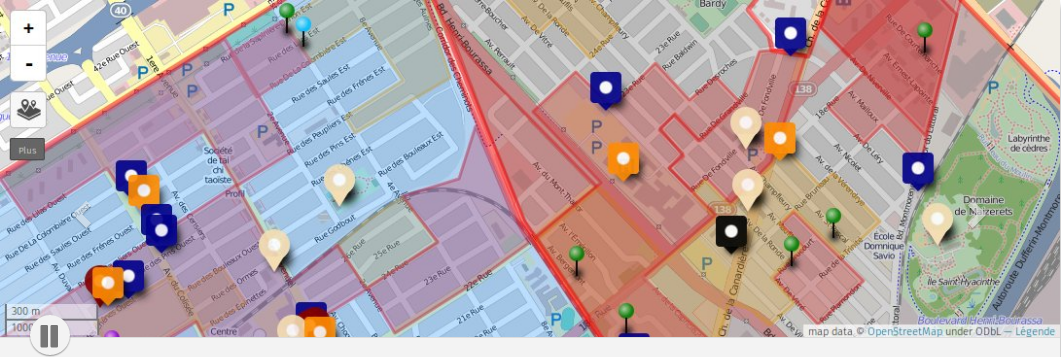
\includegraphics[width=.8\textwidth]{../pics/framacarte}
		\caption{Based on \href{https://github.com/umap-project/umap/}{uMap} and \href{https://www.openstreetmap.org}{OpenStreetMap}} 
        	\end{figure}
	\end{frame}

	\begin{frame}
	\frametitle{Framinetest $\leftrightarrow$ Minecraft}
	\framesubtitle{}
	        \begin{figure}[h]
                \centering
                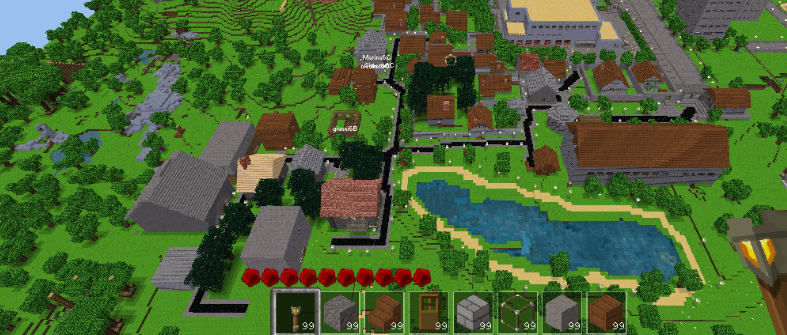
\includegraphics[width=.8\textwidth]{../pics/framinetest}
		\caption{Based on \href{http://www.minetest.net}{Minetest}}
        	\end{figure}
	\end{frame}

	\begin{frame}
	\frametitle{Framamind $\leftrightarrow$ Inspiration / Freemind}
	\framesubtitle{}
	        \begin{figure}[h]
                \centering
                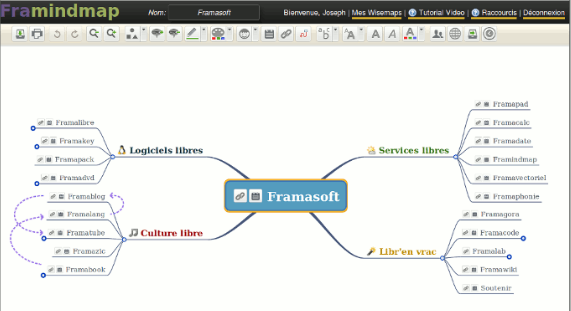
\includegraphics[width=.8\textwidth]{../pics/framamind}
        	\end{figure}
	\end{frame}

	\begin{frame}
	\frametitle{Framabookin $\leftrightarrow$ Kindle Store (for free books)}
	\framesubtitle{}
	        \begin{figure}[h]
                \centering
                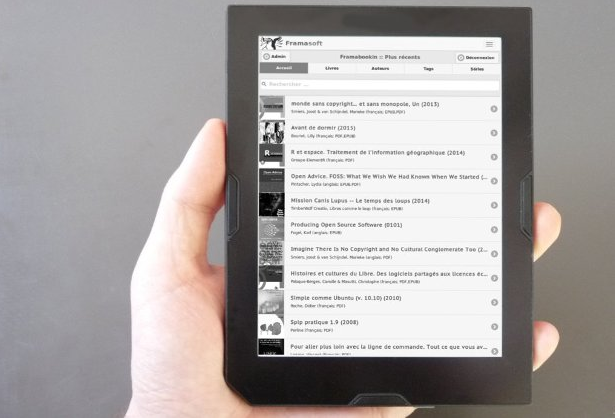
\includegraphics[width=.8\textwidth]{../pics/framabookin}
        	\end{figure}
	\end{frame}

	\begin{frame}
	\frametitle{More Software -beyond Framasoft}
	\framesubtitle{}
	\begin{columns}
		\column{0.5\textwidth}
	        	\begin{figure}[h]
               		\centering
                	
\includegraphics[width=.8\textwidth]{../pics/LF-201607}
        		\end{figure}
		\column{0.5\textwidth}
	        	\begin{figure}[h]
                	\centering
                	
\includegraphics[width=.8\textwidth]{../pics/LF-201602}
        		\end{figure}
	\end{columns}
	\end{frame}


	\frame{
		\frametitle{Conclusion}
		\begin{outline}
			\1 Find your comfortable position on the Privacy--Convenience spectrum
			\pause
			\1 Full privacy is achievable
			\pause
			\1 Most Cloud services have alternatives
			\pause
			\1 Run applications from your trusted machines
			\pause
			\1 Trust must be earned
			\pause
			\1 Work towards a more free, secure, and private world
		\end{outline}
	}



	\begin{frame}
	\frametitle{}
	\framesubtitle{}
	\centering\huge
	Feel Free\\
	Be Free!
	\end{frame}



\frame[allowframebreaks]{
	\frametitle{References}
	%\framesubtitle{References}
	% keyword refers to bib file: references-KEYWORD.bib, and to the Tex file: section-KEYWORD.tex
	\printbibliography[keyword=privacy]
}


\end{document}




\end{document}

